\section{Machine Learning Basics}
\begin{multicols}{2}
	\subsection{Capacity, Overfitting and Underfitting}
	The goal of machine learning is to perform well on data that has \textbf{never been seen before}.
	Good training results in a low training error while good \textbf{generalization} results in a \textbf{low test error}.
	In linear regression, we train with the training set for a low training error
	\[ \frac{1}{m^{\text{(train)}}} \lVert \bol{X}^{\text{(train)}}\bol{w}-\bol{y}^{\text{(train)}} \rVert_2^2 \]
	but we are really interested in the test error, which we estimate with a test set
	\[ \frac{1}{m^{\text{(test)}}} \lVert \bol{X}^{\text{(test)}}\bol{w}-\bol{y}^{\text{(test)}} \rVert_2^2 \]
	
	\textbf{Capacity} is loosely defined as the flexibility a model has to fit the data. 
	For example, for linear regression the capacity can be increased by allowing \textbf{polynomials} instead of only linear functions:
	\[ \hat{y} = b + wx \quad\rightarrow\quad \hat{y} = b + w_1x + w_2x^2 \]
	The output is still a linear function of the parameter vector $w$, hence the same normal equations derived before can be used to find the solution.
	In other words, we simply pretend that $x^2$ is also an independent input.\\
	The capacity can now simply be controlled by allowing higher and higher orders of polynomials, i.e., for order nine:
	\[ \hat{y} = b + \sum_{i=1}^{9} w_ix^i \]
	
	In general, machine learning algorithms work best, when their capacity is appropriate in regard to the true complexity of the task they need to perform and the amount of training data they are provided with.
	\begin{figure}[H]
		\centering
		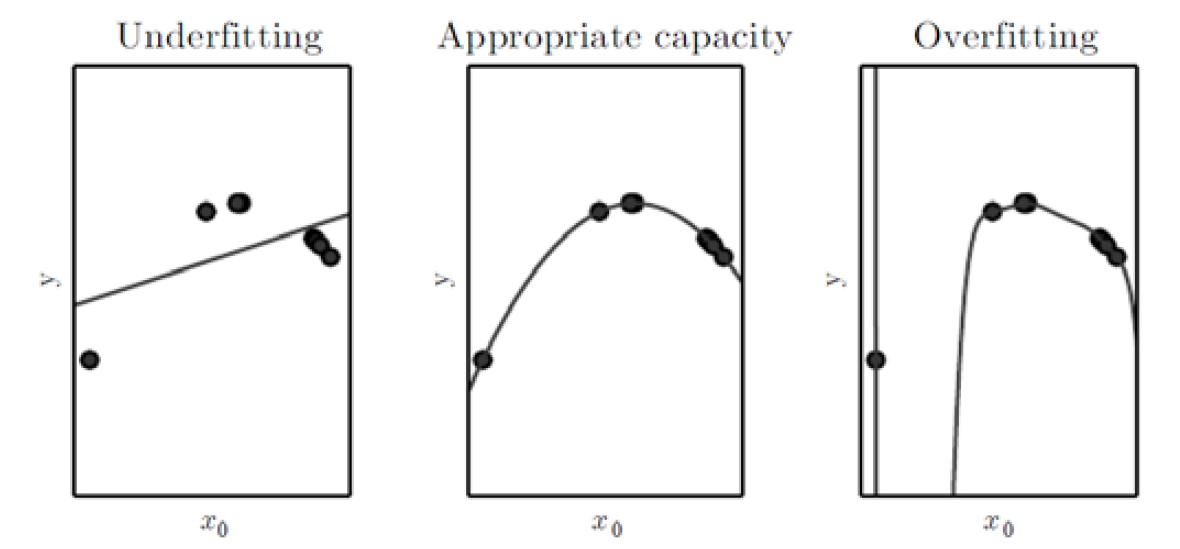
\includegraphics[width=0.85\linewidth]{images/capacity.PNG}
	\end{figure}

	While the training error will only decrease as the capacity is increased, the test error follows a U-shape curve which can be used to find the optimal capacity.
	\begin{figure}[H]
		\centering
		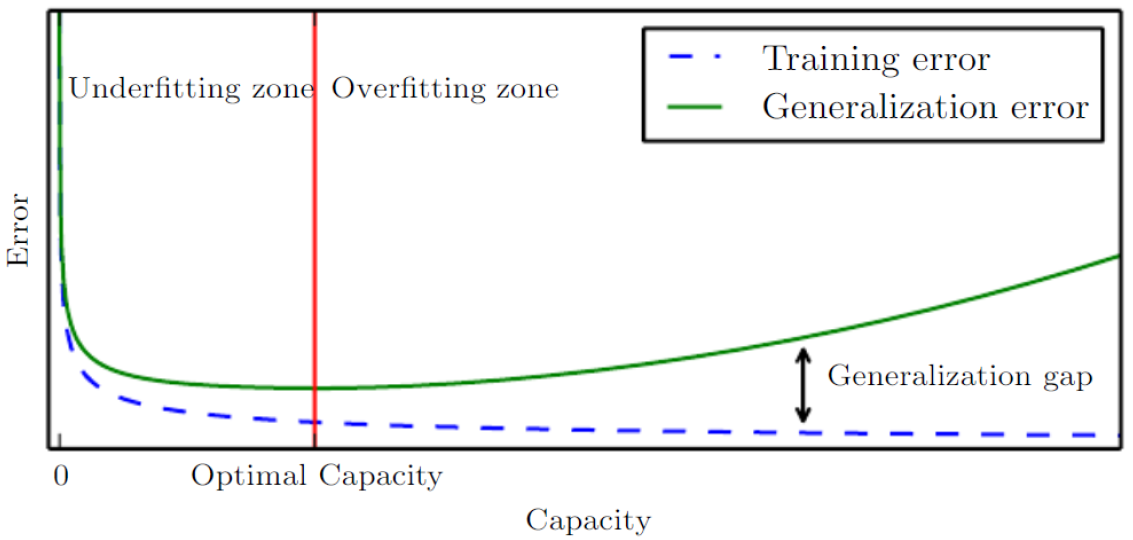
\includegraphics[width=0.95\linewidth]{images/gen_curve.PNG}
	\end{figure}
	
	The \textbf{ideal model} would know the true data generation distribution and hence could always make the optimal decision or put out the optimal value. 
	Nevertheless, in all interesting cases, the test error would not be zero, since the relationship between input $\bol{x}$ and output $y$ might be inherently stochastic or the deterministic output depends on variables that are not in the input.
	The error incurred when having access to the true distribution and making optimal use of it is called the \textbf{Bayes error} or \textbf{irreducible} error and it is the \textbf{smallest possible error}.
	
	\subsection{Regularization}
	We need to design the machine learning algorithms for the particular task at hand.
	As seen, we can try to match the capacity of the model to the complexity of the task.
	An alternative concept is to steer the algorithm towards preferred solutions.
	For example in the polynomial regression case, we might be preferring solutions that results in weights that have a small Euclidean norm squared:
	\[ J(\bol{w}) = \text{MSE}_{\text{train}} + \lambda \bol{w}^T\bol{w} \]
	This approach is called weight decay and is quite popular. 
	In linear regression this results in the well known \textbf{ridge regression} (\textbf{Tikhonov} regularization).
	If $\lambda$ is zero, then normal linear regression results.
	If $\lambda$ is very large, then the weight vector is basically zero.\\
	
	\textbf{In general}, a model that is supposed to learn a function $f()$ can be regularized by adding a penalty term called a regularizer to the cost function $f(\bol{x};\bol{\theta})$.
	For weight decay the regularizer is
	\[ \Omega(\bol{w}) = \bol{w}^T\bol{w} \]
	
	\subsection{Cross-Validation}
	If the available data set is small, then the test set is even smaller, hence estimating the test error is unreliable.
	An approach called \textbf{k-fold cross validation} can then be used to estimate the resulting test error.
	k-fold (k is usually 10) cross validation splits the data into k non-overlapping subsets. 
	Then K-1 sets are used to train and the left-out set is used to estimate the test error.
	This is repeated k times and all the test errors of each experiment are averaged.
	
	\subsection{Bias}
	The bias of an estimator is defined as
	\[ \text{bias}(\hat{\bol{\theta}}_m) = \Exp (\hat{\bol{\theta}}_m)-\bol{\theta} \]
	Estimators are considered unbiased, if the bias is zero, which implies that on average the estimator is correct.
	\[ \Exp (\hat{\bol{\theta}}_m) = \bol{\theta} \]
	A milder form is the idea of asymptotically unbiased, which means as we gather more and more data, the estimator becomes less and less biased, until in the extreme of infinitely many data points it is unbiased
	\[ \underset{m\rightarrow\infty}{\lim} \Exp (\hat{\bol{\theta}}_m) = \bol{\theta} \]
	
%	\textbf{Example: Bernoulli Distribution:}
%	\[ P(x^{(i)};\theta) = \theta^{x^{(i)}} (1-\theta)^{(1-x^{(i)})} \]
%	The goal of an estimator is to estimate the unknown mean. 
%	An obvious estimator would be the average over the training samples:
%	\[ \hat{\theta}_m = \frac{1}{m} \sum_{i=1}^{m} x^{(i)} \]
%
%	\textbf{Example: Gaussian Distribution:}
		
	\subsection{Variance and Standard Error}	
	\textbf{Sample Mean:}
	\[ \hat{\mu}_m = \frac{1}{m} \sum_{i=1}^{m} x^{(i)} \]
	
	\textbf{Standard Error:}
	\[ \text{SE}(\hat{\mu}_m) = \sqrt{\var\left[\frac{1}{m}\sum_{i=1}^{m}x^{(i)}\right]} 
	= \frac{\sigma}{\sqrt{m}} \]
		
	\textbf{MSE vs. Bias and Variance:}
	\[ \text{MSE} = \Exp\left[(\hat{\theta}_m-\theta)^2\right] = \text{Bias}(\hat{\theta}_m)^2+\var(\hat{\theta}_m) \]
		
		
	\subsection{Maximum Likelihood Estimation}
	The idea of the maximum likelihood principle is, that we pick the parameter vector is such a way, that the likelihood that the model would have generated the observed training data is maximized:
	\begin{align*}
	\bol{\theta}_{ML}
	&= \underset{\bol{\theta}}{\arg \max} p_{\text{model}} (\mathbb{X};\bol{\theta})\\
	&= \underset{\bol{\theta}}{\arg \max} \prod_{i=1}^{m} p_{\text{model}} (\bol{x}^{(i)};\bol{\theta})
	\end{align*}
	
	Usually the focus is on the \textbf{log likelihood}, since it is simpler:
	\[\bol{\theta}_{ML} = \underset{\bol{\theta}}{\arg \max} \sum_{i=1}^{m} \log p_{\text{model}} (\bol{x}^{(i)};\bol{\theta}) \]
	
	Note that we can divide the argument in the argmax() operator by $m$, and the result of the argmax operator does not change. But then we have a term where we sum up all the contributions and divide by how many there are:
	\[ \hat{p}_{\text{data}}(\bol{x}) = \frac{1}{m} \sum_{i=1}^{m} \delta(\bol{x}-\bol{x}^{(i)}) \]
	
	\subsection{Conditional Log-Likelihood and Mean Squared Error}
	In supervised learning we actually need to estimate the conditional probability $P(y|x;\bol{\theta})$.
	If we let $X$ represent all of the input and $Y$ all of the observed target, then the conditional maximum likelihood estimator is given by
	\[ \bol{\theta}_{ML} = \underset{\bol{\theta}}{\arg \max} P(\bol{Y}|\bol{X};\bol{\theta}) \]
	
	If (as it is usual) the examples are independent and identically distributed (i.i.d.) then this maximization can be written as
	\[ \bol{\theta}_{ML} = \underset{\bol{\theta}}{\arg \max} \sum_{i=1}^{m} P(\bol{y}^{(i)}|\bol{x}^{(i)};\bol{\theta}) \]
	
	\textbf{Example: Linear Regression as Maximum Likelihood estimation:}\\
	So far the goal of linear regression was to minimize the MSE.
	For maximum likelihood estimation, we need a parametrized model distribution:
	\[ p(y|\bol{x}) = \mathcal{N}\left(y;\hat{y}(\bol{x};\bol{w}),\sigma^2\right) \qquad 
	\hat{y} = \bol{w}^T\bol{x} \]
	
	Now we use the i.i.d. assumption and hence we can apply the formula
	\[ \bol{\theta}_{ML} = \underset{\bol{\theta}}{\arg \max} \sum_{i=1}^{m} P(\bol{y}^{(i)}|\bol{x}^{(i)};\bol{\theta}) \]
	
	The log of a Gaussian RV results in several additive terms and the exponent is canceled by the log.
	Hence the following results, where the parameter vector $w$ is now abstracted as parameter vector $\theta$. 
	In the formula below, this parameter vector is hidden inside of $\hat{y}$:
	\begin{align*}
	&\sum_{i=1}^{m} \log \left(y^{(i)}|\bol{x}^{(i)};\bol{\theta}\right)\\
	= &-m\log\sigma - \frac{m}{2}\log(2\pi)-\sum_{i=1}^{m}\frac{\lVert\hat{y}^{(i)}-y^{(i)}\rVert^2}{2\sigma^2}
	\end{align*}
	
	We need to now pick $\bol{w}$ in such a way, that the equation below is maximized. 
	Since the first two terms are independent of $w$, that is equivalent to minimizing the last term. 
	Since $\sigma$ is given, this is equal to minimizing the MSE!
	\[ \text{MSE}_{\text{train}}=\frac{1}{m}\sum_{i=1}^{m}\lVert \hat{y}^{(i)}-y^{(i)}\rVert^2 \]
	
	\subsection{Stochastic Gradient Descent}
	This is a direct extension to gradient descent where the expectation in gradient decent is not calculated over all examples but estimated by \textbf{using only a few sampled} examples.
	The negative conditional log-likelihood of the training data can be written as
	\begin{align*}
	J(\bol{\theta}) &= \Exp_{\bol{x},y\sim \hat{p}_{\text{data}}} L(\vx,y,\bol{\theta})\\
	&= \frac{1}{m} \sum_{i=1}^m L\left(\vx^{(i)},y^{(i)},\bol{\theta}\right)\\
	L\left(\vx,y,\bol{\theta}\right) &= -\log p(y|\vx;\bol{\theta})
	\end{align*}
	$L$ is the per-example loss. Minimizing the negative log likelihood will result in the maximum likelihood solution.
	The log over the i.i.d. samples result in the sum and the division by $m$ is added to make the expression an expectation over the empirical data distribution.\\
	The gradient of this function can be calculated as
	\[ \nabla_{\bol{\theta}}J(\bol{\theta}) = \frac{1}{m}\sum_{i=1}^{m}\nabla_\bolt L\left(\vx^{(i)},y^{(i)},\bolt\right) \]
	Clearly the larger the training set ($m$), the longer a single gradient descent step takes to calculate ($O(m)$).\\
	
	The main insight of SGD is, that the gradient is an \textbf{expectation}, which can be estimated by using a small set of samples.
	In each step of SGD a so called minibatchof samples is used, where the $m'$ samples are drawn uniformly from the training set $\sB=\{\vx^{(1)},\dots,\vx^{(m')}  \}$. The minibatch size $m'$ ranges between 1 up to maybe 1024 and is \textbf{usually a power of 2}.\\
	Since $m'$ is fixed, the size of the training set $m$ does not matter for the complexity of a SGD step anymore.
	A training set with billions of samples can be trained with minibatches with only hundreds of samples.
	Hence an estimate of the gradient is now formed, using the minibatch samples:
	\[ \bol{g} = \frac{1}{m'}\sum_{i=1}^{m'} \nabla_\bolt L\left(\vx^{(i)},y^{(i)},\bolt\right) \]
	
	Now this estimate of the gradient is used in the parameter update equation of gradient descent instead of the true gradient
	\[ \bolt \leftarrow \bolt - \epsilon \bol{g} \]
	
	\subsection{Building a Machine Learning Algorithm}
	Most deep learning algorithm have the same ingredients:
	\begin{itemize}
		\item A large data set
		\item A cost function
		\item A probabilistic model
		\item An optimization algorithm 
	\end{itemize}

	\textbf{The cost function} includes almost always a term that causes the learning process to perform some form of statistical estimation.
	Hence the most common cost function is the negative log-likelihood
	\[ J(\bol{w},b) = - \Exp_{\vx,y\sim \hat{p}_{\text{data}}} \log p_{\text{model}}(y|\vx) \]
	Minimizing the negative log-likelihood results in a maximum likelihood estimation.\\
	
	The cost function often contains additional regularization terms, for example, the weight decay term we have already seen for linear regression:
	\[ J(\bol{w},b) = \lambda\lVert \bol{w}\rVert_2^2 - \Exp_{\vx,y\sim \hat{p}_{\text{data}}} \log p_{\text{model}}(y|\vx) \]
	This implies that \textbf{weights closer to zero are preferred} over larger weights.
	In linear regression the addition of this term does still result in a closed form solution, the well known ridge regression.
	
	\subsection{Local Constancy and Smoothness Regularization}
	For algorithms to generalize well, they need to be guided by some form of prior knowledge about the problem, especially in the high-dimensional case, this is of fundamental importance.
	A very popular prior belief is the smoothness (local constancy) prior
	\[ f^\ast (\vx) = f^\ast (\vx + \epsilon) \]
	Basically, the function we try to learn should not change very much in a small neighborhood $\epsilon$.
	Many classical machine learning schemes are based on this (KNN, Trees, SVM) and as a result, they tend to fail in more complex tasks.
	Deep learning introduces additional priors in order to reduce the generalization error on more challenging tasks.\\
	Classical learning algorithms need $O(k)$ examples to distinguish $O(k)$ regions in the input space using a smoothness prior.\\

	The smoothness assumption works well in low dimensions, if there are enough training points.
	In high dimensions, the function might still be smooth, but it can change simultaneously in many dimensions.
	In addition it might behave differently in different regions.
	The function might also be quite complicated, i.e., there is a large number of regions compared to the number of examples. Is it possible to generalize in these cases?\\
	
	The answers is Yes, as long as we introduce some dependencies between the region.
	For example if we can use 2 training examples ($X_1$ and $X_2$) to define $2^2=4$ regions, if we assume as structure shown below:
	\begin{table}[H]
		\centering
		\begin{tabular}{c|c|c|}
			& $X_1$ & NOT $X_1$ \\ 
			\hline 
			$X_2$ & Region 1 & Region 2 \\ 
			\hline 
			NOT $X_2$ & Region 3 & Region 4 \\
			\hline
		\end{tabular} 
	\end{table}

	Hence this is achieved via additional assumptions about the underlying data generating distribution.
	Many deep learning algorithms provide implicit or explicit assumptions that are reasonable for a broad range of AI tasks in order to capture these advantages.
	These assumptions are much more sophisticated than the simple relationship shown in the table.\\
	
	Traditional machine learning algorithms often make stronger, task specific assumptions.
	For the checkerboard example, assuming some form of periodicity would clearly improve the generalization, but is very specific.
	In deep learning, such strong task specific assumptions are avoided, hence they often are widely applicable.
	Complex AI tasks have a much too complex structure, as that they could be captured with simple ideas like periodicity.\\
	
	\textbf{Composition of factors} is the core idea of deep learning, we assume that the data was generated hierarchically over several levels by the composition of factors.
	These mild assumptions allow for an exponential gain in the relationship between the number of training examples and the number of regions that can be distinguished.
	\begin{figure}[H]
		\centering
		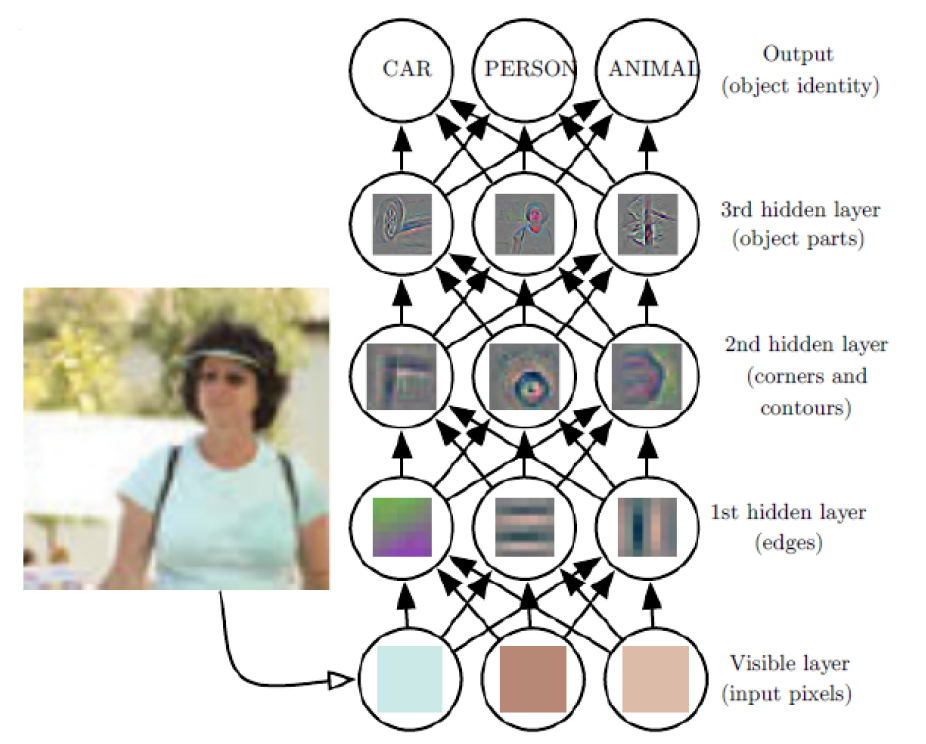
\includegraphics[width=0.75\linewidth]{images/whut.PNG}
	\end{figure}
	
	\subsection{Manifold Learning}
	A manifold is a set of points associated with a neighborhood around each point.
	From any given point, the manifold locally appears to be a Euclidean space.
	For example, we experience the surface of the world as a 2D plane but it is actually a 2D spherical manifold in 3D.
	The idea of a manifold is, that the connected set of points can be approximated well by considering only a small number of degrees of freedom, or dimensions, embedded in a higher-dimensional space. Each dimension corresponds to a local direction of variation as can be seen in the figure below.
	\begin{figure}[H]
		\centering
		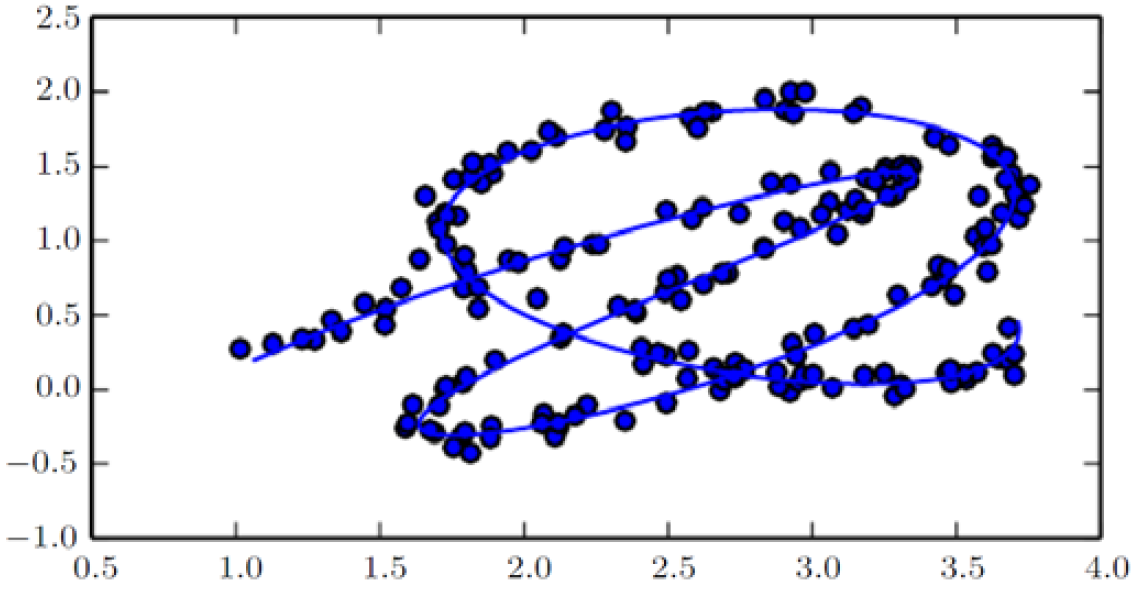
\includegraphics[width=0.75\linewidth]{images/mani.PNG}
	\end{figure}
	Now one can move from point to point along a manifold. Clearly the hope is, that these points are training samples.
	In machine learning, the dimensionality of the manifold is allowed to vary from one point to another.
	This happens for example, when the manifold has a self intersection.
	A figure \textbf{8} has a one dimensional manifold at all points, except at the intersection, where it clearly has two dimensions.
	Many problems seem arbitrarily complex, if the scheme needs to learn functions with interesting variations across all dimensions.
	In manifold learning, this is simplified by assuming that interesting inputs must lie along manifolds. Hence most inputs are not valid inputs.\\
	
	The assumption that the data lies along a low-dimensional manifold may not always be correct or useful.
	For complex AI tasks, such as computer vision, speech recognition and/or natural language processing, it appears that this manifold assumption is at least approximately correct.
	One piece of evidence, that the manifold assumption is useful for describing the probability distribution over images, text and sound, is the fact that uniform noise never resembles structured inputs from this domain.\\
	
	When the data lies on a low-dimensional manifold then it can be most natural to represent the data in terms of the coordinates of this manifold.
	For example roads are 1D manifolds in a 3D world. Addresses are in the 3D world are naturally given with respect to the 1D manifold we call road and not in 3D coordinates. Explicitly extracting these manifold coordinates is challenging, but hold the promise to improve many machine learning algorithms.
\end{multicols}
\newpage




































